\section{Models and Algorithms}\label{tes}
%--------------------------------------------------------------------------------------
\subsection{Voronoi Tessellations}\label{tes:sec:vor}
A Voronoi Diagram is a partitioning of a space $S$ by a set of points. Given $n$ points (seed points) the the space, $P = \{p_0,p_2,...,p_{n-1}\}, P \subset S$, is partitioned into $n$ regions, known as Voronoi Regions or Voronoi Cell, where every point, $s \in S_i,0 \leq i \leq n-1$ in a region, $S_i \subset S$, is closest to a single seed point, $p_i \in P$, in terms of the space's distance measurement operation, $d$ (\cite{okabe2009spatial}). An example of a Voronoi Diagram can be seen in Figure \ref{tes:fig:voreg}.
%
\subsubsection{Weighted Voronoi Tessellations}\label{tes:ssec:wei}
%
\subsubsection{Voronoi Tessellations in Non-Euclidean Spaces}\label{tes:ssec:warp}
%--------------------------------------------------------------------------------------
\begin{figure}[H]
	\centering
    \label{tes:fig:voreg}
    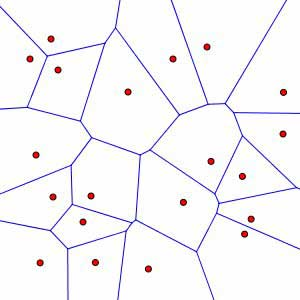
\includegraphics[scale=0.65]{Images/voronoi.jpg}
    \caption{Voronoi Diagram(\cite{voronoipic})}
\end{figure}
%--------------------------------------------------------------------------------------
\subsection{Voronoi Tessellation Generation Algorithms}\label{tes:sec:tga}
Although Voronoi Tessellations extend to multiple dimensions, for the sake of these algorithms we will only discuss those in a two dimensional plane.
%
\subsubsection{Incremental Algorithm}\label{tes:ssec:inc}
The most simplistic of the generation algorithms, the Incremental is an iterative algorithm as described by \cite{green1978computing} and \cite{okabe2009spatial}.
\begin{enumerate}
\item Starting from $i=0$ and an empty plane
\item\label{tes:itm:inc:add} A seed point, $p_i$ is placed into the plane.
\item The nearest neighboring seed point $p_f=p_{nn}$ is found
\item\label{tes:itm:inc:bis} A perpendicular bisector is drawn between $p_i$ and $p_f$ (if it exists).
\item The bisecting line is followed in both directions until it intercepts an existing edge or the plane's boundary on both ends.
\item A new edge is defined by this segment of the bisector as part of both $p_i$ and $p_f$.
\item The seed point of the polygon that shares the found edge clockwise to $p_f$ (anticlockwise to $p_i$) is then set to $p_f$.
\item Continue from step \ref{tes:itm:inc:bis} until $p_f=p_{nn}$ again.
\item Set $i = i +1$ and repeat from step \ref{tes:itm:inc:add} until $i=n$
\end{enumerate}
In it's most naive form, this algorithm achieves and efficiency of $O(n^2)$.
%
\subsubsection{Divide and Conquer Algorithm}\label{tes:ssec:dac}
The Divide and Conquer algorithm was first proposed by \cite{shamos1975closest} and also described in \cite{okabe2009spatial}. It is a recursive algorithm which improves on the Incremental algorithm by having a construction time of $O(n\log n)$.
\begin{enumerate}
\item If the  contains only one point, return it with the entire plane as it's voronoi region.
\item Divide the space, $S$ containing the set of seed points, $P$ with $n$ points, into two subspaces, $S_L$ and $S_R$, such that $S_L$ and $S_R$ contain $n/2$ seed points and every seed point of $P_L$ lies to the left of every seed point of $P_R$ (this is made easier if $P$ is ordered).
\item Recursively compute the voronoi tessellations for $P_L$ in $S_L$ and $P_R$ in $S_R$; $V_L$ and $V_R$ respectively.
\item A polygonal line, $Q$, must now be found such that $Q$ merges $V_L$ and $V_R$ into a single voronoi tessellation, $V$:
\begin{enumerate}
 \item Starting with the polygon of $V_R$ which contains the top-left corner of $S_R$, $p_R$ and the polygon of $V_L$ which contains the top-right corner of $S_L$, $p_L$. Since $p_L$ must lie to the left of $p_R$, they must overlap when $V_L$ and $V_R$ are extended into $S$.
 \item\label{tes:itm:dac:bis} A perpendicular bisector is drawn between $p_L$ and $p_R$ and segmented between its two closest edge intercepts from the shortest distance between $p_L$ and $p_R$ and add this segment to $Q$.
 \item If the lower intercepting edge of the is in $V_R$ then $p_R$ is set to the seed point polygon which shares this edge and similarly if the edge is in $V_L$.
 \item Continue from step \ref{tes:itm:dac:bis} until the bottom of $S$ is reached.
\end{enumerate}
\item Remove all line segments of $V_L$ to the right of $Q$ and all those of $V_R$ to the left of $Q$ to form $V$.
\item Return $V$ recursively until the full voronoi tessellation is complete.
\end{enumerate}
Part of achieving this efficiency is assuming $P$ is co-lexicographically ordered, meaning for all $p_i,p_j \in P$, $0 \leq i < j < n$; $x_i > x_j$ or $(x_i = x_j$ and $y_i > y_j)$. This speeds up the partitioning of $P$ into $P_R$ and $P_L$ at each level of recursion.
%
\subsubsection{Fortune's Algorithm (Sweep-Line Method)}\label{tes:ssec:fort}
\cite{fortune1987sweepline} describes an algorithm where the tessellations are found by a line ``sweeping'' over the space and solving the problem at each step of the sweep. This can be problematic for Voronoi tessellations as the line may intercept the Voronoi Region of a seed point before it intercepts the point. Therefore the Voronoi Tessellation is not computed directly, but through a geometric transform. The transform $\phi(x(s),y(s))$ works such that for any point, $s \in S$ with coordinates $(x(s),y(s))$, 
\begin{equation}
  \phi(x(s),y(s)) = (x(s) + r(s), y(s))
\end{equation}
Where $r_i(s)$ is defined as the distance to the seed point $p_i \in P$ and $r(s) = min\{r_i(s) | 1 \leq i \leq n-1\}$, is the distance to the closest seed point to $s$. This transform can then easily be reversed to re-obtain $S$ and its set of Voronoi tessellations. Now, for the transform of $S$, $\phi(S)$ denoted by $\Phi$, the left-most point of each Voronoi Region is its seed point (except the left-most seed point), this is essential for the algorithm. It is important to note that the perpendicular bisectors of seed points in $S$, through the transform, become hyperbola in $\Phi$ (provided they are not horizontal in $S$). For $p_i,p_j\in P$, the hyperbola is denoted as $h_{ij}$ which can be split into $h^+_{ij}$ and $h^-_{ij}$ as the upper and lower parts about the left-most point respectively. Set $Q$ is denoted as the set of all event points in the algorithm. $Q$ is initially populated with the seed points (in co-lexicographical order) but the edge interceptions will be added as they are found. The algorithm, as described by \cite{okabe2009spatial} goes as follows:
\begin{enumerate}
\item Add $P$ to $Q$.
\item Choose and delete the leftmost seed point, $p_i$ from $Q$
\item Create a list, $L$ containing the transformed voronoi region of $p_i$, $\phi(V_i)$.
\item While $Q$ is not empty repeat steps \ref{tes:itm:for:w}, \ref{tes:itm:for:seed} and \ref{tes:itm:for:line}.
\begin{enumerate}
  \item\label{tes:itm:for:w} Choose and delete the leftmost element, $w$ of $Q$.
  \item\label{tes:itm:for:seed} If $w$ is a seed point:
  \begin{enumerate}
    \item Set $w=p_i$.
    \item Find the region, $\phi(V_j)$, containing $p_i$.
    \item Replace $\phi(V_j)$ in $L$ with $(\phi(V_j),h^-_{ij},\phi(V_i),h^+_{ij},\phi(V_j))$
  \end{enumerate}
  \item\label{tes:itm:for:line} If $w$ is a half-edge:
  \begin{enumerate}
    \item 
  \end{enumerate}
\end{enumerate}
\end{enumerate}

%--------------------------------------------------------------------------------------
\subsection{Clustering Algorithms} \label{tes:sec:clu}
%
\subsubsection{K-Means Algorithm}\label{tes:ssec:kma}
%--------------------------------------------------------------------------------------
\subsection{Related Works}\label{ra:sec:rel}
%
\subsubsection{Naive Method}\label{ra:ssec:nm}
%
\subsubsection{Standard Voronoi Model}\label{ra:ssec:svm}
%--------------------------------------------------------------------------------------
%--------------------------------------------------------------------------------------